% !TEX root = ../ausarbeitung.tex
%%% DELETE THIS LATER
%Im Hauptteil beschreiben Sie Ihre praktische Arbeit. Code gehört %normalerweise nicht in eine Ausarbeitung. Ausnahmen sind Algorithmen, %die für Sie wichtig waren (dann in möglichst übersichtlichem Pseudo-%Code). Kleine Code-Stücke können auch zur Illustration oder als Beispiel %eingebaut werden. Längere Code-Stücke können im Anhang %untergebracht werden. Sie sollten jedoch nicht den gesamten Code im %Anhang abdrucken. Ihren Code geben Sie bitte dennoch mit ab, am %besten auf einer CD.
%
%Der Detailgrad sollte so sein, dass ein Leser die gleiche Arbeit noch %einmal nachimplementieren könnte. Insbesondere sollten alle Parameter, %von denen die Funktionsweise des Systems abhängt, explizit genannt %sein. Bei der Evaluation muss bei jedem Versuch angegeben werden, mit %welchen Parametern gearbeitet wird.
\chapter{Herangehensweise}
In diesem Kapitel wird der Weg von der Konzipierung mehrerer Konzepte für das Lernspiel bis zur Implementierung des Spiels behandelt.
\section{Konzeptwahl des Spiels}
\subsection{Erste Idee Math Smashers}
Die erste Idee ein Lernspiel zu entwickeln, welches Grundschüler unterstützt die Addition über das Konzept der Partnerzahlen zu lernen war das bereits vorhandene Spiel \textit{Math Smashers}.\\
In \textit{Math Smashers} fliegen Bälle mit Zahlen herum. Als Spieler kann man eine Art Seil zwischen 2 Kugeln anbringen. Dieses Seil zieht sich zusammen um die Kugeln zu einer zusammen zu fassen. Dabei werden beide Zahlen addiert. Ziel ist es alle Bälle so zu addieren, damit man die gesuchte Zahl heraus bekommt. Dabei kann es vorkommen mehrmals die gesuchte Zahl zu bekommen.
\begin{figure}[htb]
	\centering
	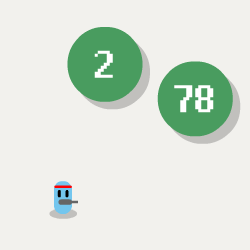
\includegraphics[width=0.3\textwidth]{MathSmasher-NotConnected}
	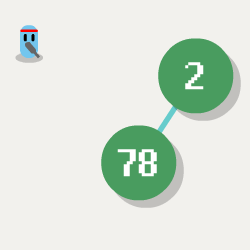
\includegraphics[width=0.3\textwidth]{MathSmasher-Connected}
	\caption{MathSmashers links 2 nicht verbundene Zahlen. Rechts beide Zahlen verbunden\label{fig:mathsmashers}}
\end{figure}
\subsection{Weitere Ideenfindung}
Zunächst wurden weitere Ideen erarbeitet, wie das Konzept der Partnerzahlen noch in einem Spiel untergebracht werden kann. Dabei entstanden die folgenden 4 Ideen.
\subsubsection{Kombination mit The Legend of Zelda} %TODO Ref!
Diese Idee war als Anlehnung an das Spiel The Legend of Zelda gedacht. Kombiniert wurde es mit dem bereits beschriebenen Math Smashers. In diesem Fall hat man statt Bällen die aus The Legend of Zelda: Majoras Mask bekannten Schleimgegner allerdings mit Zahlen darin. Ziel ist es auch hier 2 Zahlen zu einer gesuchten zu addieren, indem man Schleimgegner mit den passenden Partnerzahlen besiegt und die im Schleim liegenden Zahlen addiert.
%TODO Grafik einfügen
\begin{figure}[htb]
	\centering
	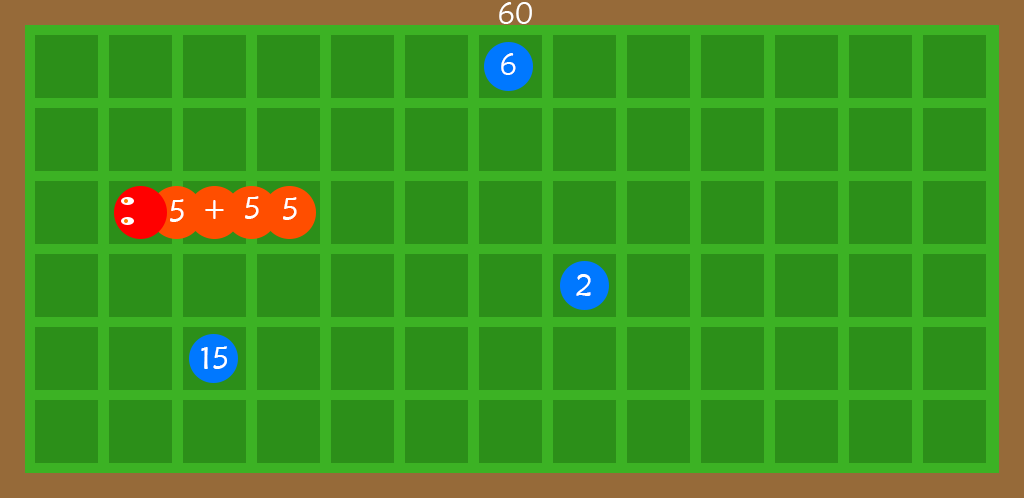
\includegraphics[width=0.75\textwidth]{Snake-Skizze}
	\caption{Skizze der Legend of Zelda Idee\label{fig:zelda}}
\end{figure}
\subsubsection{MathSnake}
Für diese Idee wurde das Addieren von Partnerzahlen zu einer gesuchten Zahl auf Snake übertragen. In diesem Snake gibt es Zahlenäpfel. Frisst die Schlange einen dieser Äpfel hat sie einen Teil der Partnerzahl gefressen und zur Addition hinzugefügt. Frisst sie den nächsten Apfel werden beide Zahlen addiert. Natürlich wird die Schlange pro Apfel länger und schneller.
\begin{figure}[htb]
	\centering
	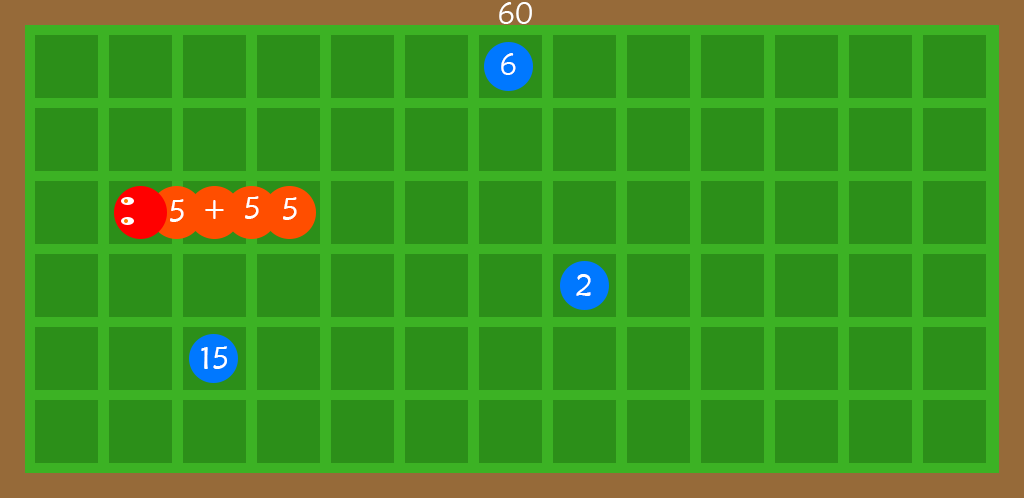
\includegraphics[width=0.75\textwidth]{Snake-Skizze}
	\caption{Skizze des MathSnake Spiels\label{fig:mathsnake}}
\end{figure}
\subsubsection{Murmeladdierer}
Diese Idee überträgt das Vorhaben auf ein altes Murmelspiel. Es gibt mehrere Löcher - mit Zahlen beschriftet - in die man Kugeln hinein bewegen muss. Die Bewegung der Kugeln wird erzielt durch das Kippen der Fläche in eine bestimmte Richtung. Wie in jedem Ansatz wird hier eine gesuchte Zahl bereit gestellt. Da zwei Kugeln gleichzeitig auf dem Feld zu bewegen sehr schwer sein könnte, kann man das ganze auch sequenziell mit jeweils einer Kugel spielen.
%TODO Grafik einfügen
\begin{figure}[htb]
	\centering
	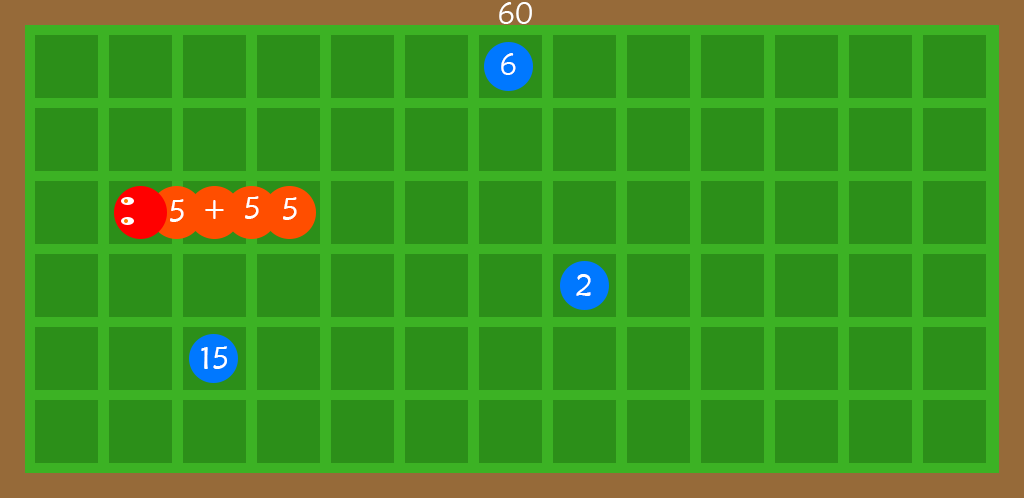
\includegraphics[width=0.75\textwidth]{Snake-Skizze}
	\caption{Skizze des Murmeladdierer Spiels\label{fig:murmadd}}
\end{figure}
\subsubsection{Zahlenbausteine}
Auch für diese Idee ist es wieder nötig Zahlen zu einer gesuchten Zahl zu addieren. Hier sind die Zahlen in Form von Ziegelsteinen gegeben und man hat ein Gebäude, welches mehrere dieser Ziegelsteine benötigt. Diese sind mit den gesuchten Zahlen beschriftet. Der Spieler muss sich dann zwei Steine auf dem Spielfeld suchen und diese aufeinander legen um sie zum gesuchten Ziegelstein zu addieren. Dieser muss dann vom Spieler an die richtige Position im Bauwerk gebracht werden.
%TODO Grafik einfügen
\begin{figure}[htb]
	\centering
	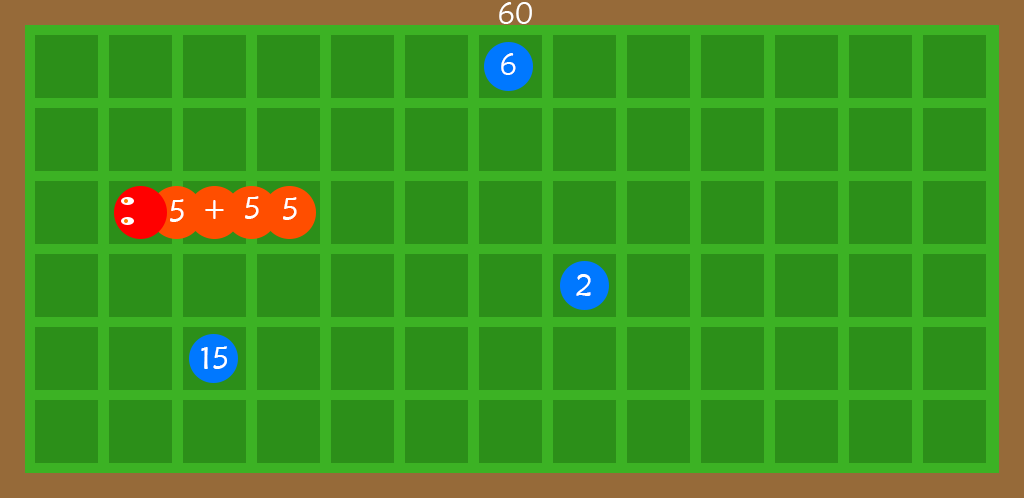
\includegraphics[width=0.75\textwidth]{Snake-Skizze}
	\caption{Skizze des Zahlenbaustein Spiels\label{fig:baustein}}
\end{figure}
\section{Wahl des Spielkonzepts und Entwicklung des Spiels}
Letzten Endes wurde die MathSnake Variante umgesetzt, da sie einem klassischen Spiel einen neuen Reiz verleiht. Die Kombination mit The Legend of Zelda würde dies ebenfalls erfüllen, allerdings würde eine Umsetzung hier erheblich mehr Zeit in Anspruch nehmen, die dann für die Evaluation gefehlt hätte. Außerdem bietet die MathSnake Variante mehr Möglichkeiten das Spiel herausfordernder zu gestalten. Zum Beispiel durch Anstieg der Bewegungsgeschwindigkeit nach dem essen eines Apfels und die Längenzunahme der Schlange. Aber auch durch weitere Features, wie dem verfaulen der Äpfel über Zeit, lässt sich das Spiel schwieriger gestalten. Diese Aspekte waren ausschlaggebend um sich für die Snake Variante zu entscheiden.
MathSnake wurde in der Entwicklungsumgebung von Unity umgesetzt. Als Zielplatform wurde Android gewählt um das Spiel auf einem Tablet spielen zu können. Um den Fokus in der Entwicklung mehr auf die Spielmechaniken zu legen wurde ein Asset-Pack aus dem Unity Asset Store verwendet. Durch dieses gab es bereits Grafiken für die Schlange und Gestaltungsdetails für die Umgebung. Die Umgebung selbst wurde in Blender modeliert und in Unity mit den gegebenen Details geschmückt.
\subsection{Verschiedene Spielversionen}
Im Zuge dieser Bachelorarbeit wurden 2 verschiedene Varianten umgesetzt und evaluiert. Zur Auswahl standen folgende Versionen mit deren erwarteten Vor- und Nachteilen.

%TODO Als Tabelle umsetzen!
\subsubsection{3D Snake mit Third-Person-Perspektive}
\textbf{Vorteile}
\begin{itemize}
\item moderner
\item mehr das Gefühl als Spieler die Schlange zu sein
\item Spielfeld kann Abwechslungsreich gestaltet werden mit mehreren Ebenen
\item Übersicht auf welcher Ebene man sich befindet ist sehr gut
\item Um einfach Zahlen zu sammeln gut, da die Zahl erst gesucht werden muss und man nicht direkt weiß wo die beste Zahl liegt
\end{itemize}
\textbf{Nachteile:}
\begin{itemize}
\item wenig Übersicht über das Spielfeld, welche Zahlen wo liegen ist nicht gegeben.
\end{itemize}
\subsubsection{3D Snake mit TopDown-Perspektive}
\textbf{Vorteile}
\begin{itemize}
\item moderner
\item Spielfeld kann mit unterschiedlichen Ebenen gestalltet werden.
\item Gute Übersicht darüber wo welche Zahl liegt
\end{itemize}
\textbf{Nachteile:}
\begin{itemize}
\item Übersicht über die aktuelle Ebene auf der man sich bewegt kann verwirren?
\end{itemize}
\subsubsection{2D Snake mit TopDown-Perspektive}
\textbf{Vorteile}
\begin{itemize}
\item einfache Umsetzung
\item Gute Übersicht darüber wo welche Zahl liegt
\item Grafisch nicht so aufwändig
\end{itemize}
\textbf{Nachteile:}
\begin{itemize}
\item nicht viel neues zu lernen
\item weniger Möglichkeiten um den Spieler herauszufordern
\end{itemize}
\subsubsection{Snake mit Grid}
\textbf{Vorteile}
\begin{itemize}
\item Einfache Steuerung
\item Einfach um neue Objekte in die Spielwelt zu legen
\item Objekte können nicht ineinander liegen
\end{itemize}
\textbf{Nachteile:}
\begin{itemize}
\item weniger Freiheiten für den Spieler, da nur 4 Richtungen
\item weniger Freiheiten im Leveldesign -> muss quadratisches Spielfeld sein
\end{itemize}
\subsubsection{Snake ohne Grid}
\textbf{Vorteile}
\begin{itemize}
\item moderne Steuerung
\item Spieler hat kann sich in mehrere Richtungen bewegen
\item Leveldesign kann durch verschiedene Formen unterstützt werden
\end{itemize}
\textbf{Nachteile:}
\begin{itemize}
\item Objekte können ineinander liegen (Aufwändiger dies abzufangen)
\item Aufwändiger den "Spawnbereich" zu definieren
\end{itemize}

Entschieden wurde sich dann für die beiden 3D Varianten ohne Grid, da das Ziel war beide Versionen vergleichen zu können um zu ermitteln, welche Version bei Spielern besser ankommt. Außerdem konnten wir so für beide Versionen die gleichen Grafiken verwenden. So blieb der Fokus auf der unterschiedlichen Perspektive auf das Spielgeschehen. Ebenfalls wurde sich gegen ein Grid, also eine Einteilung in mehrere Felder, auf denen sich die Schlange bewegt, entschieden um eine modernere Steuerung für Snake umzusetzen.
\section{Aufbau und Funktionsweise des Spiels}
\subsection{Aufbau des Spiels}
\subsubsection{Menüführung}
Der Aufbau des Spiels ist sehr einfach gehalten. Der Spieler beginnt das Spiel im Hauptmenü, welches in Abbildung \ref{fig:mathsnake-menu} dargestellt wird. In diesem kann er sich für eine Spielversion entscheiden, die Highscore Tabelle begutachten oder das Spiel beenden. Startet er eine der beiden Spielversionen beginnt direkt das Spiel. 
%TODO Skizze der Menüführung
\begin{figure}[htb]
	\centering
	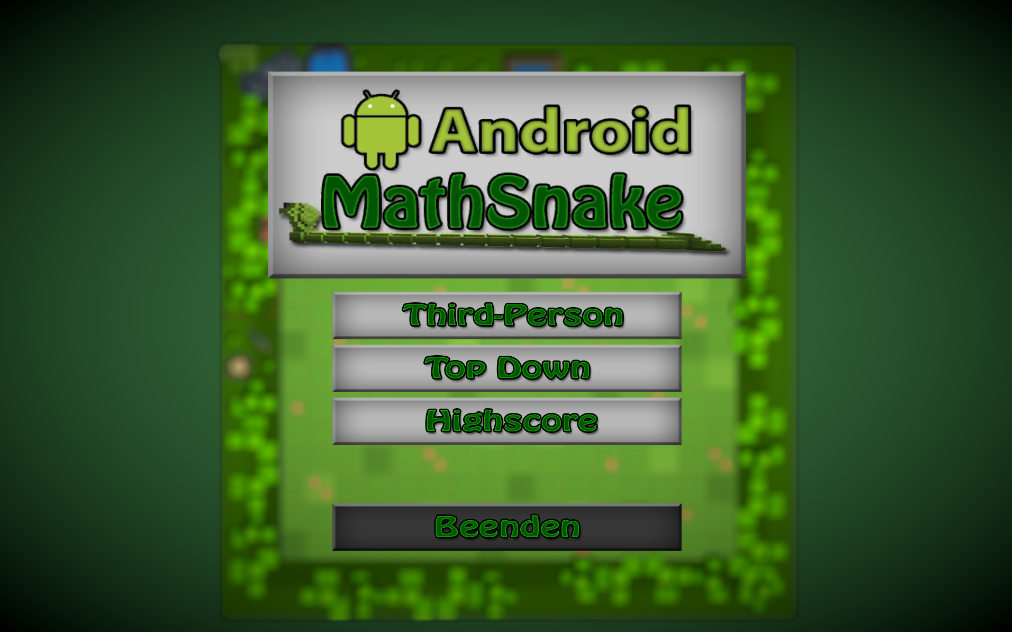
\includegraphics[width=0.65\textwidth]{MathSnake-MainMenu}
	\caption{Hauptmenü von MathSnake\label{fig:mathsnake-menu}}
\end{figure}
\subsubsection{Spielfeldaufbau}
Der Spieler sieht am oberen Bildschirmrand die gesuchte Zahl gefolgt von einem '='. Auf dieses folgen dann alle gefressenen Zahlen mit einem '+' verbunden. Dies stellt die Gleichung dar, die erfüllt sein muss um die Aufgabe zu bestehen. Links neben der gesuchten Zahl findet der Spieler auch seinen aktuellen Score. Dieser nimmt bei einer falschen Zahl ab und bei einer richtigen Zahl zu. Der Spieler kann die Schlange über zwei Pfeiltasten steuern. Diese zwei Tasten geben die Richtung an in die sich die Schlange bewegen soll. Der Spieler kann sie über diese Tasten also nach rechts oder links bewegen. 
%TODO Bild des Spiels mit Beschriftung
\subsubsection{Highscore}
Das Spiel stellt auch eine simple Highscore Liste breit um weiteren Anreiz zu schaffen. Dieser wurde allerdings für den Nutzertest deaktiviert, da die Nutzer sich voll auf die Bewertung des Spiels an sich konzentrieren sollten und der Highscore nicht Teil der Forschungsfragen war.\\
Ist der Highscore aktiviert, wird einem nach dem Ende einer Spielrunde eine Nachricht angezeigt ob man genügend Punkte gesammelt hat um sich in der Highscore Liste eintragen zu können. Dies geschieht dann über ein Textfeld in dessen man Name eingeben soll, wie in Abbildung \ref{fig:mathsnake-newHighscore} zu sehen ist.
\begin{figure}[htb]
	\centering
	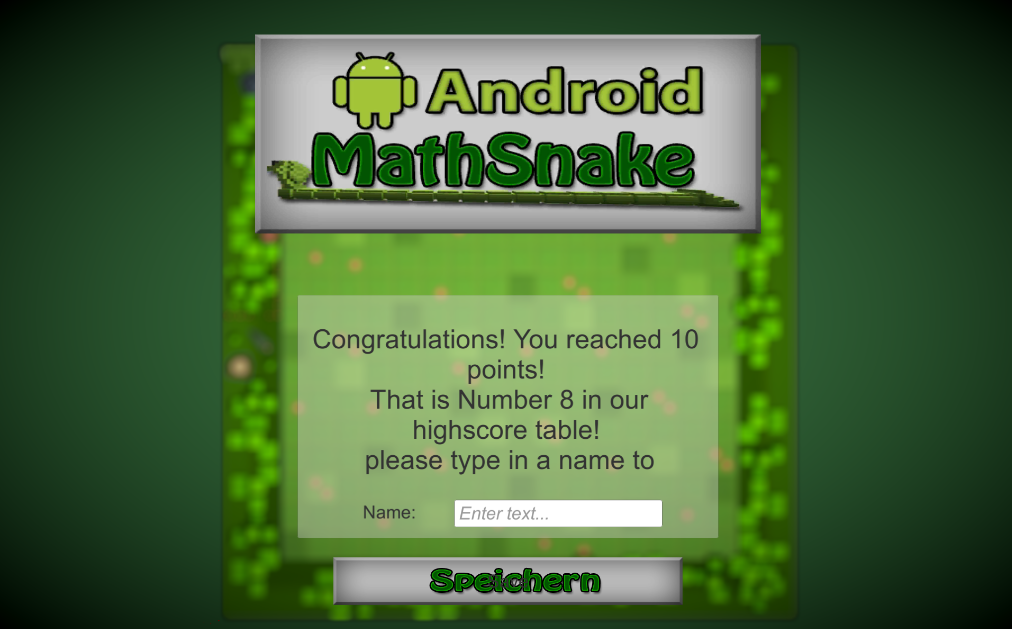
\includegraphics[width=0.65\textwidth]{MathSnake-Highscore1}
	\caption{Erstellen eines neuen Highscore-Eintrags\label{fig:mathsnake-newHighscore}}
\end{figure}
Im Hauptmenü kann dann, wie in Abbildung \ref{fig:mathsnake-menu} zu erkennen ist, die aktuelle Highscore-Tabelle angezeigt werden. Diese ist so aufgebaut, dass Platz 1 mit der höchsten Punktzahl oben steht. Gibt es Spieler mit der gleichen Punktzahl schlägt ein neueres Ergebnis ein älteres. In Abbildung \ref{fig:mathsnake-HighscoreTable} ist eine Beispielhafte Ansicht der Highscore-Tabelle abgebildet.
\begin{figure}[htb]
	\centering
	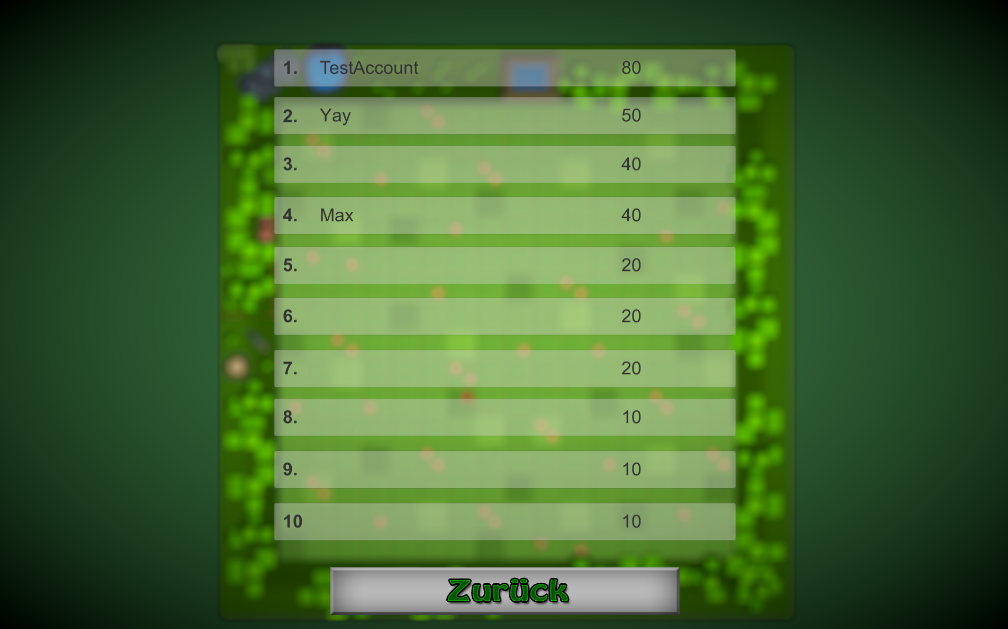
\includegraphics[width=0.65\textwidth]{MathSnake-Highscore2}
	\caption{Ansicht der Highscore-Tabelle\label{fig:mathsnake-HighscoreTable}}
\end{figure}
\subsection{Funktionsweise des Spiels}
Das entwickelte Spiel lässt sich nun entweder in der TopDown Ansicht oder in der ThirdPerson Ansicht spielen. Die Funktionsweise bleibt bei beiden identisch. Der Spieler steuert eine Schlange und kann diese mit zwei Pfeiltasten nach rechts oder links drehen um die Bewegungsrichtung zu verändern. Am oberen Bildschirmrand wird ihm eine gesuchte Zahl angezeigt sowie seine aktuelle Punktzahl. Hat er einen Apfel mit einer Zahl gefressen erscheint diese neben der gesuchten Zahl als Gleichung. Pro gegessenem Apfel wird die Schlange schneller und länger.
\begin{figure}[htb]
	\centering
	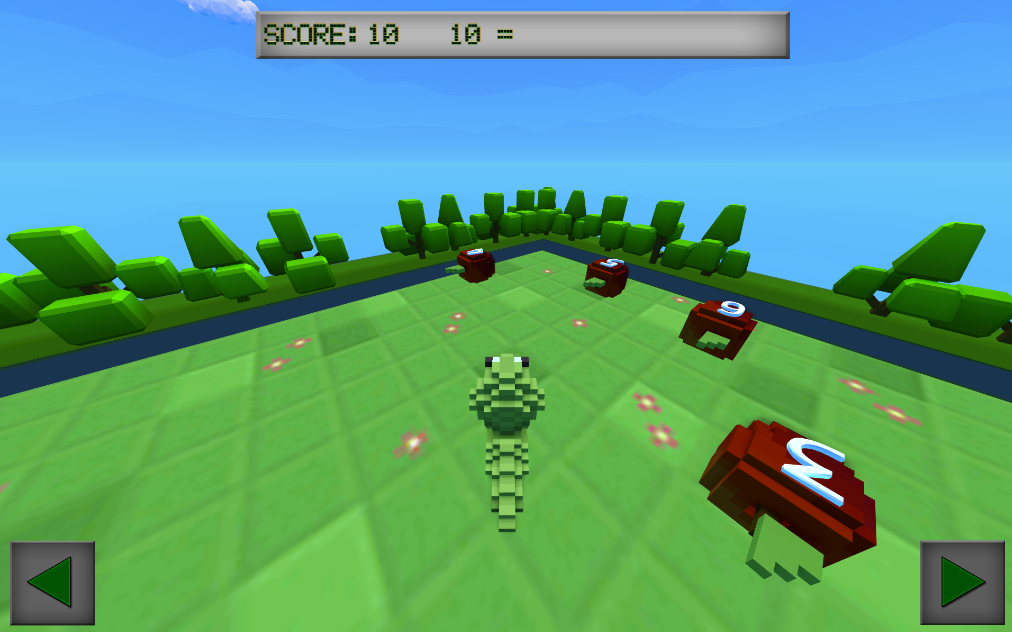
\includegraphics[width=0.35\textwidth]{MathSnake-ThirdPerson}
	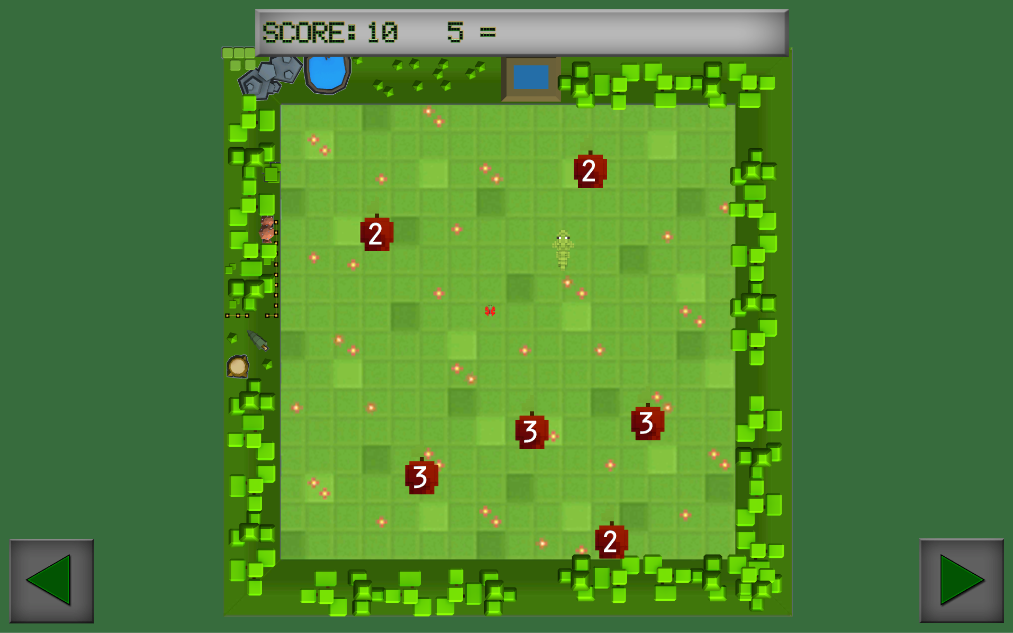
\includegraphics[width=0.35\textwidth]{MathSnake-TopDown}
	\caption{ThirdPerson und TopDown Perspektiven\label{fig:mathsnake-perspektives}}
\end{figure}
\subsubsection{Levelsystem}
Pro zu suchende Zahl gibt es ein Level. Um das Spiel auf Dauer herausfordernder zu gestalten, wurde ein kleines Levelsystem eingeführt. Dabei varriiert der Zahlenraum je nachdem in welchem Levelbereich man ist. Im höchsten Bereich beginnen die Äpfel zu verfaulen. In der Tabelle \ref{tab:levels} ist die implementierte Zuordnung zu entnehmen.
\begin{table}[h!]
\centering
\begin{tabular}{|l|l|l|}
\hline
\textbf{Level} & \textbf{Zahlenbereich} & \textbf{Eigenschaften}       \\ \hline
0-4            & 3-20                   & -                            \\ \hline
5-9            & 20-50                  & -                            \\ \hline
10-19          & 50-100                 & -                            \\ \hline
20-49          & 30-100                 & -                            \\ \hline
50+            & 30-100                 & Äpfel verfaulen mit der Zeit \\ \hline
\end{tabular}
\caption{Bedeutung der einzelnen Levelbereiche\label{tab:levels}}
\end{table}
\newpage
\subsubsection{Ansicht auf das Spielgeschehen}
Wie bereits beschrieben wurde für das Spiel jeweils eine Version mit TopDown Ansicht und eine Version mit ThirdPerson Ansicht implementiert. Während die erste Version das klassische Snake mit Ansicht aus der Vogelperspektive ist, ist die zweite Version ein modernerer Ansatz. Bei der ThirdPerson Ansicht positioniert man die Kamera direkt hinter dem Schlangenkopf. Das Spielprinzip an sich bleibt in beiden Versionen gleich.


